\subsectionA{Scrab}
Scrabs are small, insectoid men that live in nests in the desert. A scrab can draw air through sand while submerged due to the long gills located all along the grooves in their shells. Scrabs are ruled over by monstrously bloated members of the species known as nest mothers.

Scrabs need very little water to survive and seem to derive all the sustenance that they need from the blood and other bodily fluids of their victims.

Scrabs can speak their own language. A small percentage can also speak elvish. Adult scrabs live to be 25 years old, but nest mothers can live twice that long.

\begin{figure}[t!]
\centering
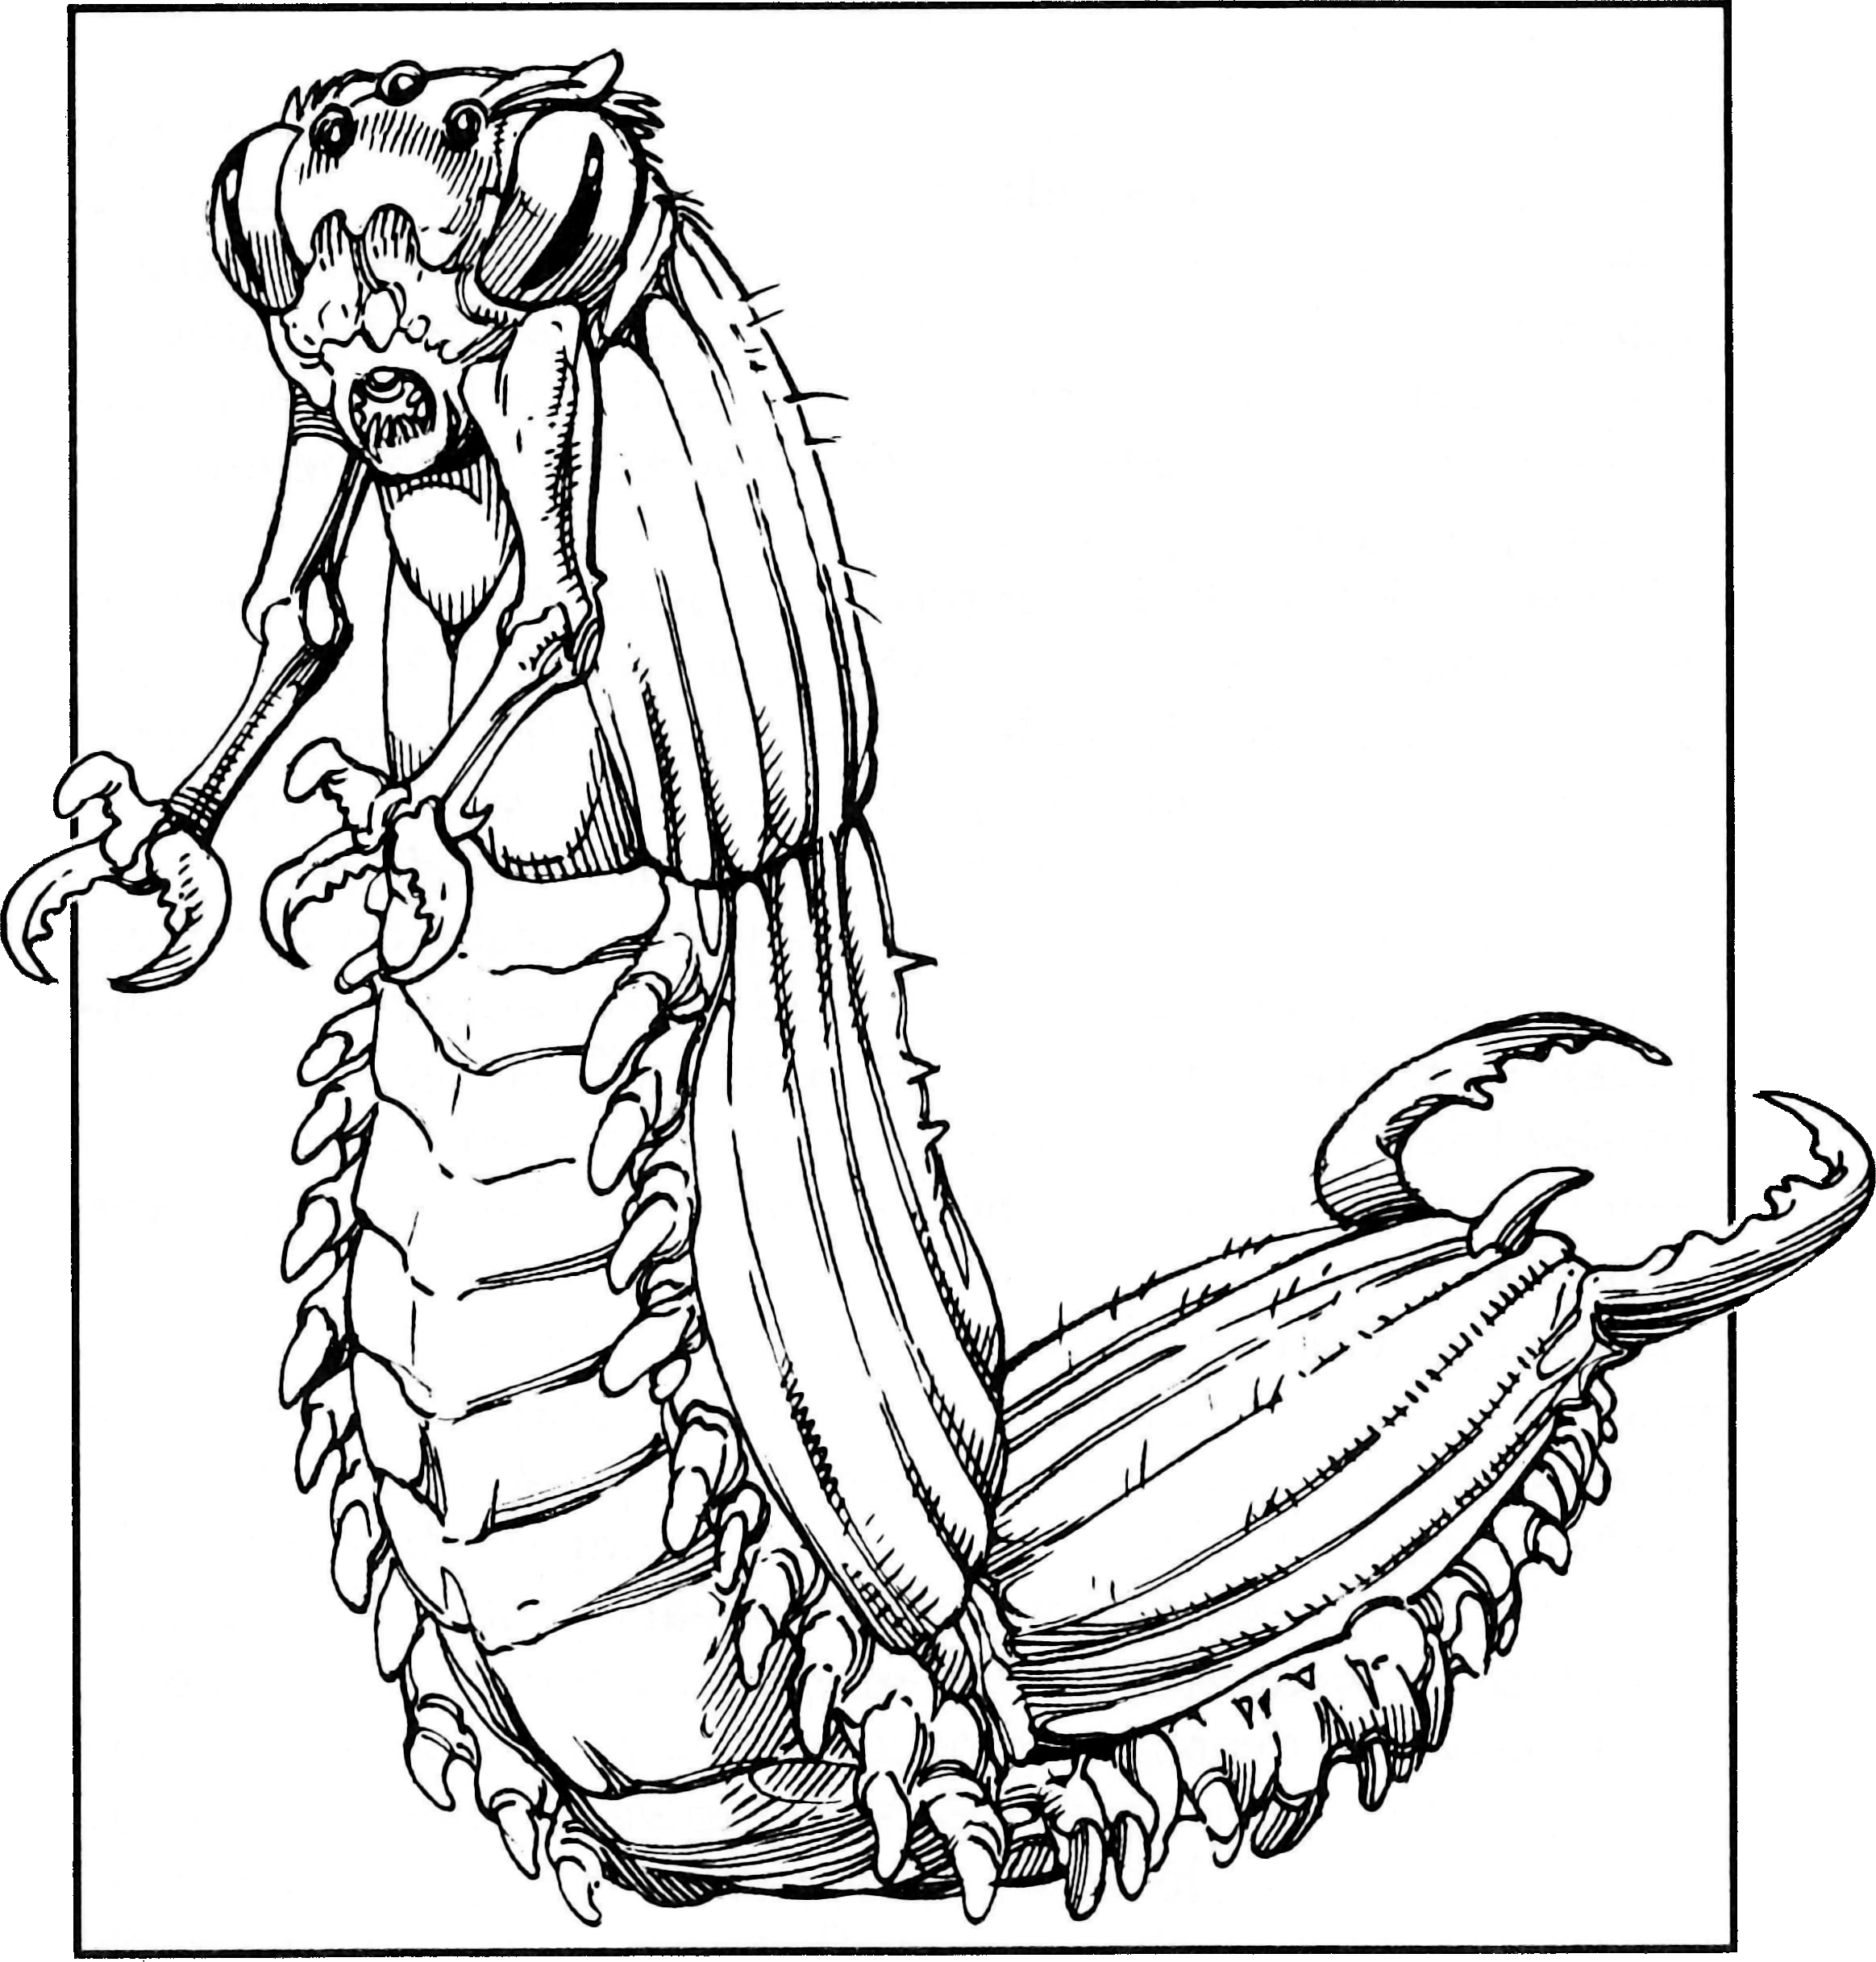
\includegraphics[width=\columnwidth]{images/scrab.png}
\WOTC
\end{figure}

\subsubsection{Scrab Society}
Scrabs inhabit tunnels deep under the desert, which they fashion using spittle that solidifies the sand. If possible, the entrance to the nest will be concealed behind a rocky outcrop. Scrabs hate elves and prefer their flesh above that of any other creature. This hatred extends beyond a desire for food and, in fact, anything with pointed ears is likely to be identified as an elf. A captive elf may be kept alive for weeks, even months, just to be tortured. Legends of both races hold that there were once great wars between the two species, with each side blaming the other for the conflicts and for the many unspeakable atrocities perpetrated on innocent victims of each race.

The eldest male in the nest is allowed to mate with the nest mother, with clutches of up 100 eggs resulting. The eggs hatch in three months, and the young are possessed by a cannibalistic frenzy when they are born. Fewer than half the hatchlings survive this period. Three quarters of all hatchlings are male.

Only males who develop additional psionic abilities or spellcasting powers grow into leaders, and only females with clerical abilities can become nest mothers. A female who begins to develop into a nest mother will take a number of males and depart to create a new nest of her own.

Scrabs are predators first and foremost but will trade with merchants brave enough to risk contact with the creatures. They are also preyed upon by the larger creatures that inhabit the wastes. Part of the scrabs' hatred of elves stems from the fact that elves use every part of a scrab they have defeated. A scrab shell can be used to make breastplates, and the sharp parts of the pincers make decent polearms.

\subsubsection{Scrab Racial Traits}
\begin{itemize*}
    \item +4 Intelligence, +2 Wisdom.
    \item Monstrous Humanoid: Scrabs are not subject to spells or effects that affect humanoids only, such as \spell{charm person} or \spell{dominate person}.
    \item Small. Scrabs gain a +1 size bonus to Armor Class, a +1 size bonus on attack rolls, and a +4 size bonus on \skill{Hide} checks, but they must use smaller weapons than humans use, and their lifting and carrying limits are three-quarters of those of a Medium character.
    \item A scrab's base land speed is 15 meters. Scrabs also have a burrow speed of 3 meters.
    \item Darkvision: Scrabs can see in the dark up to 18 meters. Darkvision is black and white only, but it is otherwise like normal sight, and scrabs can function just fine with no light at all.
    \item Racial Hit Dice: A scrab begins with 5 levels of monstrous humanoid, which provide 5d8 Hit Dice, a base attack bonus of +5, and base saving throw bonuses of Fort +1, Ref +4 and Will +4.
    \item Racial Skills: A scrab's monstrous humanoid levels give it skill points equal to 8 $\times$ (2 + Int modifier). Its class skills are \skill{Concentration}, \skill{Hide}, \skill{Listen}, \skill{Move Silently}, \skill{Psicraft}, \skill{Spot}, and \skill{Survival}.
    \item A scrab's monstrous humanoid levels give it 2 feats.
    \item Weapon Proficiency: A scrab is proficient with its natural weaponry and all simple weapons.
    \item Natural Armor: +5 natural armor bonus to AC.
    \item Natural Weapons: 2 claws (1d4).
    \item Improved Grab: To use this ability, a scrab must hit with a claw attack. It can then attempt to start a grapple as a free action without provoking an attack of opportunity. If it wins the grapple check, it deals automatic claw damage each round it remains grappling.
	\item Psionic Powers: A scrab character manifests psionic powers as a 5th-level psion. If the character takes additional levels of psion, these levels stack with the scrab's base manifesting ability for powers known, power points per day, and other effects dependent on manifester level. A scrab character likewise uses the sum of its racial spellcasting levels and class levels to determine the abilities of its psicrystal.
    \item Automatic Languages: Scrab. Bonus Languages: Common, Elven, Entombic.
    \item Favored Class: Psion.
    \item Level Adjustment: +3.
\end{itemize*}
